\chapter{Implementation}
\label{chap:implementation}

\section{Software Architecture}
\label{sec:impl_architecture}

The conformal uncertainty quantification framework is implemented as a Python package, \texttt{volatility\_smoothing/conformal/}, together with the experiment notebook. It operates as a post-hoc layer around the pre-trained GNO, whose architecture and weights are not modified. The implementation constructs masked GNO inputs, receives predictions at held-out target locations, and returns calibrated prediction bands. The package is structured into six modules, each covering one part of the pipeline described in Chapter~\ref{chap:methodology}. Table~\ref{tab:modules} lists the main interfaces and their roles.

\begin{table}[ht]
\centering
\small
\begin{tabularx}{\textwidth}{|>{\raggedright\arraybackslash}p{0.27\textwidth}|>{\raggedright\arraybackslash}p{0.29\textwidth}|X|}
\hline
\textbf{Module} & \textbf{Primary interface} & \textbf{Role} \\
\hline
\texttt{nonconformity\_scores.py} & \texttt{SpreadNormalizedScore} & Score A: spread-normalised price error \\
                                  & \texttt{VegaNormalizedScore}  & Score B: Vega-weighted IV error \\
\hline
\texttt{rolling\_window.py}       & \texttt{RollingWindowCalibration} & FIFO window of target scores from the $L$ most recent surfaces \\
\hline
\texttt{mondrian.py}              & \texttt{MondrianConformal}    & Spatial binning and per-bin quantile computation \\
\hline
\texttt{prediction\_bands.py}     & \texttt{PredictionBands}      & Band construction in price-spread and Vega-IV modes \\
\hline
\texttt{no\_arbitrage\_projection.py} & \texttt{project\_band\_surfaces\_fixed\_k} & Joint fixed-$k$ calendar and discrete butterfly adjustment of both band surfaces \\
\hline
\texttt{evaluation.py}            & \texttt{build\_masked\_gno\_input} & Context/target masking, GNO query construction, and surface-level bootstrap summaries \\
\hline
\end{tabularx}
\caption{Main modules of the \texttt{volatility\_smoothing/conformal/} package and their roles.}
\label{tab:modules}
\end{table}

The modules are wired together in \texttt{conformal\_prediction.ipynb}, which is the integration point for the reported experiment and is described in Section~\ref{sec:impl_notebook}. The notebook also defines the exact conformal order statistic, the final Score B weighting and band helper, and the reported projection diagnostics. Each component is described below.

\section{Nonconformity Score Computation}
\label{sec:impl_scores}

Both nonconformity scores are implemented in \texttt{nonconformity\_scores.py} as subclasses of a common \texttt{NonconformityScore} base class. Its \texttt{compute} method accepts the GNO predictions, the corresponding market implied volatilities, and the auxiliary market data required by the score. The dispatcher \texttt{compute\_scores\_from\_data} selects the scorer from the \texttt{score\_type} argument. In the final experiment, it receives only the held-out target subset and the GNO predictions at those target locations.

Score A (\texttt{SpreadNormalizedScore}) works in price space. It takes three steps: (1) compute predicted and market prices from the corresponding implied volatilities using the Black-Scholes formula in transformed coordinates - $d_1 = -z/v + v\rho/2$ and $d_2 = -z/v - v\rho/2$, with call and put prices handled separately based on the sign of the log-moneyness $k = \rho z$, (2) read bid and ask prices directly from the dataloader as dollar-denominated quantities and floor the spread at $0.10$, (3) divide twice the absolute price residual by the floored spread, per Equation~\ref{eq:score_a}. When the market-price reference is the bid--ask midpoint and the observed spread exceeds the floor, a score below 1 indicates that the model price lies within the observed bid--ask interval. More generally, the score measures the price residual relative to the floored spread.

Score B (\texttt{VegaNormalizedScore}) works directly in implied volatility space. The notebook helper \texttt{score\_from\_data} computes forward-normalised Vega at the observed market implied volatility, divides it by the mean market-IV Vega over the held-out target set, and multiplies the absolute IV residual by the resulting relative weight. The completed ratio $\mathcal{V}/\bar{\mathcal{V}}$ is floored at \texttt{min\_weight}$=1.0$, so options with above-average Vega are up-weighted and no option is weighted below 1. This calibration definition is distinct from the prediction-time plug-in weight: because the target market IV is then unknown, \texttt{vega\_iv\_bands} evaluates Vega at the GNO-predicted IV when converting the conformal quantile into a band width.

\section{Rolling Window Calibration}
\label{sec:impl_rolling}

The rolling window is implemented in \texttt{rolling\_window.py} as a \texttt{RollingWindowCalibration} class that maintains an ordered list of \texttt{CalibrationSurface} dataclasses. Each entry stores the target $(\rho,z)$ coordinates and target nonconformity scores from one market snapshot. The window operates as a FIFO buffer of fixed size $L$: \texttt{add\_surface} appends a new surface and discards the oldest if the list exceeds $L$ entries. \texttt{get\_calibration\_data} concatenates the target coordinates and scores currently in the window for global and Mondrian quantile computation. The window counts available snapshots rather than elapsed time.

Two state queries are available: \texttt{is\_ready} returns true as soon as at least one surface has been added, and \texttt{is\_full} returns true once the window has reached capacity $L$. In the experiment pipeline, quantile computation begins immediately after the first surface is added, so the Mondrian calibration runs on a growing window during the early calibration surfaces and on a full window of $L$ surfaces thereafter.

\section{Mondrian Spatial Binning}
\label{sec:impl_mondrian}

Mondrian binning is implemented in \texttt{mondrian.py} as a \texttt{MondrianConformal} class. At initialisation, the domain $D = (0.01, 1) \times (-1.5, 0.5)$ is partitioned into a regular $B_\rho \times B_z$ grid of \texttt{MondrianBin} objects using evenly spaced edges along each axis. Each bin stores the target nonconformity scores from the rolling window that fall within its boundaries.

Calibration proceeds in two passes. The final experiment uses \texttt{ExactOrderStatisticMondrian}, a subclass defined in \texttt{conformal\_prediction.ipynb}, to apply the finite-sample conformal order statistic in Equation~\ref{eq:quantile}. First, the global quantile is computed over all scores in the window as a fallback. Second, per-bin quantiles are computed for bins that contain at least \texttt{min\_samples\_per\_bin} $= 10$ scores; bins below this threshold are assigned the global quantile directly. For bins that meet the threshold, the raw bin quantile is shrunk towards the global quantile by a factor $\lambda$:
\begin{equation}
    q_{\text{bin}} = \lambda\, \hat{q}_{1-\alpha} + (1 - \lambda)\, q^{\text{raw}}_{\text{bin}},
\end{equation}
with $\lambda = 0.3$ in the experiments of Chapter~\ref{chap:results}. This prevents bins that marginally exceed the minimum count from producing extreme quantile estimates while preserving the spatial adaptivity of well-populated bins.

At evaluation time, \texttt{get\_quantiles} assigns each target point the quantile of the bin containing its $(\rho,z)$ coordinates. Points outside the domain boundaries receive the global quantile. Bin lookup uses \texttt{np.searchsorted} on the precomputed bin edges.

\section{Prediction Band Construction}
\label{sec:impl_bands}

Band construction is provided by \texttt{prediction\_bands.py} through the \texttt{PredictionBands} class. It accepts the GNO target predictions, the per-target global or Mondrian conformal quantiles, and the market data required by the chosen mode, and returns lower and upper bounds in IV and price space. In the final pipeline, Score A uses \texttt{PredictionBands.compute}, while Score B uses the notebook helper \texttt{vega\_iv\_bands}. The prediction-time weighting differs from the calibration weighting: calibration evaluates Vega at the observed market IV, whereas band construction evaluates it at the GNO-predicted IV because the target market IV is unavailable at prediction time.

Under the Vega-IV mode, the helper takes four steps: (1) compute forward-normalised Vega at each target using the GNO-predicted IV, (2) form the relative weight $w_V = \mathcal{V}/\bar{\mathcal{V}}$ over the target set and floor it at \texttt{min\_vega}$=1.0$, (3) divide the per-target conformal quantile by the weight to obtain the IV half-width $h_v = q/w_V$, and (4) subtract and add $h_v$ from the GNO prediction to obtain $v_{\text{lo}}$ and $v_{\text{hi}}$, with $v_{\text{lo}}$ clipped at $10^{-4}$. Price bands are recovered by evaluating the Black-Scholes formula at the two IV endpoints.

Under the price-spread mode, \texttt{compute} takes three steps: (1) compute the GNO predicted price using the Black-Scholes formula, (2) read bid and ask prices from the dataloader and floor the spread at \texttt{min\_spread}$= 0.10$, (3) add and subtract the price half-width $h_P = (q/2) \cdot s$ from the predicted price to get $P_{\text{lo}}$ and $P_{\text{hi}}$. IV bands are then obtained by inverting the Black-Scholes price at each endpoint via \texttt{implied\_volatility\_from\_price}, which root-finds per point using Brent's method over the interval $[10^{-4}, 5.0]$. Points where no sign change is found within this interval are clipped to the nearest bound rather than raising an error.

One important distinction is that the \texttt{black\_scholes\_price} function in this module produces dollar-denominated prices - that is, $\text{discount} \times \text{forward} \times \text{BS}(\tau, k, v)$ - rather than the forward-normalised, dimensionless $\text{BS}_\pm(x, v)$ used in Chapter~\ref{chap:methodology}. These currency units are used consistently with the observed bid and ask prices in Score A. Score B is constructed directly in implied-volatility space using the forward-normalised Vega weights described above.

\section{No-Arbitrage Projection}
\label{sec:impl_projection}

The no-arbitrage projection is implemented in \texttt{no\_arbitrage\_projection.py}. The final notebook uses \texttt{check\_butterfly\_arbitrage}, \texttt{check\_calendar\_arbitrage\_fixed\_k}, and \texttt{project\_band\_surfaces\_fixed\_k}. The scattered target-band values are represented on a rectangular grid whose rows correspond to the available target $\rho$ values, with maturities $\tau=\rho^2$, and whose columns contain 50 evenly spaced $z$ values. The mapping uses linear interpolation from \texttt{scipy.interpolate.griddata}, with nearest-neighbour interpolation outside the convex hull.

The two check functions each return an \texttt{ArbitrageConstraints} dataclass recording the violation count and maximum violation magnitude. \texttt{check\_butterfly\_arbitrage} implements the discrete butterfly check. It iterates over each maturity slice, computes total variance $w=v^2\tau$ across the $z$ direction, and flags a middle grid point when its total variance exceeds the linearly interpolated value between its two neighbours by more than a tolerance $\varepsilon=10^{-6}$. \texttt{check\_calendar\_arbitrage\_fixed\_k} compares consecutive maturity rows at the same log-moneyness $k=\rho z$. For a longer-maturity grid coordinate $z_j$, the matching shorter-maturity coordinate is $\rho_{i+1}z_j/\rho_i$ and its total variance is obtained by linear interpolation.

\texttt{project\_band\_surfaces\_fixed\_k} expresses the fixed-$k$ calendar condition and the discrete butterfly condition as sparse linear inequalities in total variance. It then calls \texttt{scipy.optimize.linprog} with the HiGHS solver to minimise the sum of absolute changes from the original lower and upper grids. Both surfaces are solved together, with positive total variance and lower/upper ordering included as additional constraints. Before conversion back to implied volatility, values that fall marginally below the small positive variance floor because of numerical solver tolerance are set to that floor, and the number of these adjustments is recorded. The function returns the projected surfaces together with the initial and final violation counts, solver status, iteration count, projection distance, floor-adjustment count, and crossing count.

The corrected grid values are mapped back to the target $(\rho,z)$ coordinates through a second \texttt{scipy.interpolate.griddata} call. A target outside the grid convex hull retains its corresponding pre-projection endpoint. The resulting values form the final $\tilde{v}_{\text{lo}}$ and $\tilde{v}_{\text{hi}}$ used for coverage and band-width evaluation in Chapter~\ref{chap:results}. Lower/upper crossings are counted after mapping back.
\section{Data Acquisition and Preprocessing}
\label{sec:impl_data}

The SPX option chains used in the empirical study were collected through the OpenBB Python interface using its Cboe provider and the symbol \texttt{SPX} \cite{openbb2026options}. A scheduled retrieval script requested the available option chain and saved the returned expiration dates, strikes, option types, bid prices, and ask prices as CSV files. The files were written in the column format expected by the existing \texttt{WRDSOptionsDataset} loader. The name of this loader therefore refers to the compatible file schema and does not imply that the observations were obtained from WRDS.

During this transformation, the calendar date on which the retrieval completed was stored in the \texttt{date} field. The dates used to order the surfaces in the notebook and figures are consequently collection dates rather than separate exchange-provided quote timestamps. The \texttt{am\_settlement} field was set to one as a compatibility field required by the loader's filtering step; it is not used in this thesis as an empirical classification of the settlement convention of each individual contract. After loading, the existing preprocessing pipeline computes the time to maturity, forward price, discount factor, log-moneyness, and implied volatility and restricts the observations to the transformed GNO domain.

The raw directory contains 56 files. Ten files whose stored dates do not correspond to a regular Cboe trading session are excluded from the analysis: eight have weekend dates, while 25 December 2025 and 3 July 2026 are exchange holidays. The 24 December 2025 early-close file is retained. The original files are not deleted; an explicit date list filters the dataset index in memory before the GNO dataset is constructed. This leaves 46 analysis surfaces with collection dates from 11 December 2025 to 11 August 2026.

The audit found no duplicate rows or duplicate contract keys within a file and no completely identical files. The 25 December file repeats the bid and ask values of the contracts also present on 26 December; excluding the non-regular-session file prevents both snapshots from entering the analysis. The retained collection dates are irregular because no successful file is available for every scheduled date. Provider API and integration errors occurred during collection, but the available logs do not identify the cause of every missing date. The CSV files also do not contain the provider quote timestamp, retrieval time, or time zone, so the stored dates are used only to order the available snapshots.

\section{Context and Target Construction}
\label{sec:impl_masking}

The masking helpers are implemented in \texttt{evaluation.py}. For each retained surface, \texttt{stratified\_context\_target\_indices} assigns approximately 20\% of the quotes to the target set within each cell of the same $4\times4$ $(\rho,z)$ partition used for Mondrian calibration. The random generator uses seed $2026+i$ for surface index $i$. A cell containing only one quote remains in the context set, and assertions verify that the context and target indices are non-empty, disjoint, and together contain every quote.

\texttt{build\_masked\_gno\_input} passes only the context features and context IV values through the GNO input arrays \texttt{x} and \texttt{pos\_x}. It appends the target coordinates to \texttt{pos\_y} as query locations and rebuilds the graph edges, without adding target IV values to the model input. \texttt{read\_masked\_gno\_output} then separates the target predictions from the GNO's regular-grid outputs. The target subset is passed to the score, band, coverage, width, and point-error calculations. Score A and Score B use the same indices on every surface.

\section{Experiment Notebook}
\label{sec:impl_notebook}

The experiment notebook \texttt{conformal\_prediction.ipynb} is the integration point for the reported pipeline. It loads the pre-trained GNO checkpoint and the WRDS-compatible OpenBB files through \texttt{WRDSOptionsDataset} and \texttt{GNOOptionsDataset}, applies the ten-date filter, and divides the 46 retained surfaces into 15 initial calibration surfaces and 31 walk-forward evaluation surfaces. The fixed settings used in the final run are listed in Table~\ref{tab:hyperparams}.

\begin{table}[H]
\centering
\begin{tabular}{|l|l|l|}
\hline
\textbf{Hyperparameter} & \textbf{Symbol} & \textbf{Value} \\
\hline
Coverage level          & $1 - \alpha$    & $90\%$ \\
\hline
Rolling window size     & $L$             & $5$ surfaces \\
\hline
Mondrian bins           & $B_\rho \times B_z$ & $4 \times 4$ \\
\hline
Shrinkage factor        & $\lambda$       & $0.3$ \\
\hline
Min samples per bin     &                 & $10$ \\
\hline
Held-out target fraction &                & $20\%$ \\
\hline
Mask base seed          &                 & $2026$ \\
\hline
Surface bootstrap resamples &             & $2{,}000$ \\
\hline
Surface bootstrap seed &                  & $2026$ \\
\hline
\end{tabular}
\caption{Fixed settings used in the final experiment.}
\label{tab:hyperparams}
\end{table}

The pipeline is encapsulated in \texttt{run\_conformal\_pipeline}, which accepts \texttt{'vega'} for Score B or \texttt{'spread'} for Score A. Each of the 15 initial calibration surfaces is masked, the GNO predicts its target points from the context observations, and the resulting target scores are added to the rolling window. During walk-forward evaluation, the global and Mondrian quantiles are first obtained from the preceding window. The GNO then predicts the current target points, the two band variants are constructed and projected, and the target coverage, width, point-prediction error, fixed-$k$ calendar and discrete butterfly counts, and lower/upper crossings are recorded. Only after this evaluation are the current target scores added to the rolling window. The function is run once for each score with identical masks.

The main coverage and width summaries first calculate one value for each of the 31 evaluation surfaces and then average those values, giving equal weight to each surface. The reported 95\% bootstrap intervals use \texttt{surface\_bootstrap\_mean\_ci} with 2{,}000 resamples and seed 2026. Each resampling unit is a complete evaluation surface rather than an individual quote.

Figure~\ref{fig:dataset_overview} shows the 46 retained surfaces. The first 15 surfaces, from 11 December 2025 to 17 February 2026, form the initial calibration set, while the remaining 31 surfaces, from 3 March to 11 August 2026, are evaluated in walk-forward order. Each retained surface contains between 8{,}677 and 11{,}325 quotes, with a mean of 10{,}119. The context sets contain 6{,}943 to 9{,}058 points and the held-out target sets contain 1{,}734 to 2{,}267 points.

\begin{figure}[H]
    \centering
    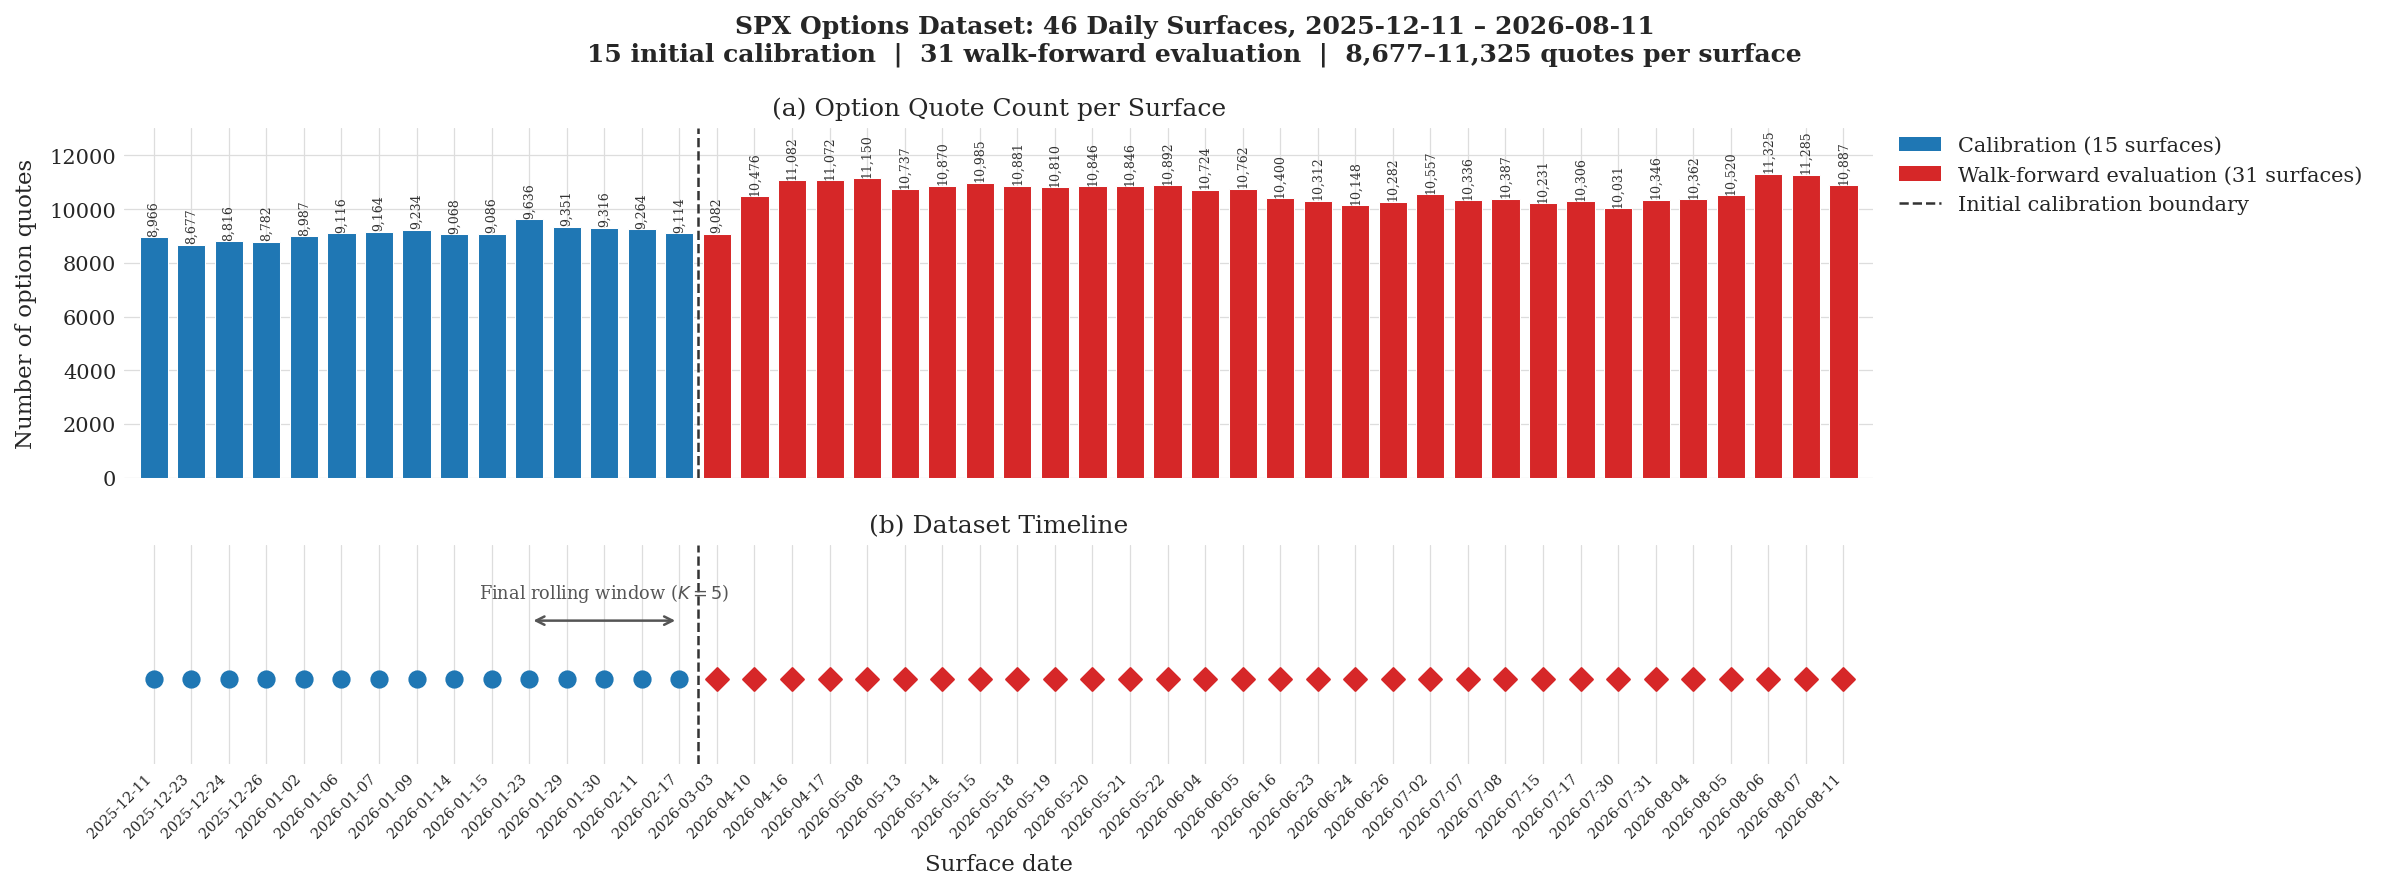
\includegraphics[width=\textwidth]{Figures/fig_dataset_overview.png}
    \caption{The 46 retained SPX option surfaces after the regular-session-date filter. Blue indicates the 15 initial calibration surfaces (indices 0--14), and red indicates the 31 walk-forward evaluation surfaces (indices 15--45).}
    \label{fig:dataset_overview}
\end{figure}
